\chapter{Resultater}\label{chapter:resultater}
I det følgende afsnit, bliver resultaterne fra komprimering af Lena med hhv. DCT og PCA præsenteret. Resultaterne vil i afsnit \ref{sec:vurdering} blive brugt til at sammenligne de to komprimeringsmetoder.

I forhold til den opstillede case er det interressant at kigge på forskellige parametre: komprimeringsgrad og billedekvalitet. Disse parametre er interessante, da det ønskes at nedbringe filstørrelsen, så en mobilbruger har plads til flere billeder på telefonen af gangen. Ydermere ønskes det, at brugeroplevelsen ikke skal påvirkes af komprimeringen, hvilket imidlertid betyder, at billedekvaliteten skal bibeholdes mest muligt.

Der er med hhv. DCT og PCA lavet test med forskellige grader af komprimering, hvor alle parametre er blevet målt med henblik på sammenligning af DCT og PCA som komprimeringsmetoder. Komprimeringer med DCT er lavet med følgende $Q$-værdier: $10$, $25$, $50$, $75$ og $90$. PCA-komprimeringerne er målt med følgende antal principale komponenter: $1$, $5$, $10$, $15$, $20$, $25$, $50$, $75$, $100$, $150$, $200$ og $512$. \\
Der tages først udgangspunkt i komprimeringsgraden for de forskellige komprimeringer.

\section{Komprimeringsgrad}
Først ses der nærmere på DCTs og PCAs evne til at komprimere den originale fil til en mindre fil. Filstørrelsen for DCT måles i bitrepræsentationen fra en TXT-fil, der er Huffmankodet. Det er dermed ikke TXT-filens faktiske størrelse, da fokusset i dette projekt har været på matematikken bag komprimeringen og ikke datastrukturen i en binær fil. Ligeledes måles filstørrelsen af de PCA-komprimerede filer ved den totale længde af bitrepræsentationen i filen. \\
Den oprindelige filstørrelse betragtes som værende det totale antal pixels i alle farverum multipliceret med otte, da hvert tal repræsenteres med otte bit. Dette giver en filstørrelse på $512\cdot512\cdot3\cdot8 = 6.291.456$ bit for det oprindelige billede. Komprimeringsgraden er beregnet som $$\text{Komprimeringsgrad} = \frac{\text{Oprindelig filstørrelse}}{\text{Komprimeret filstørrelse}}$$
Tabel \ref{tb:komprimering_DCT}, \ref{tb:komprimering_PCA1} og \vref{tb:komprimering_PCA2} præsenterer komprimeringsgraden for de forskellige komprimeringer med de to metoder.
\begin{table}[htbp]
\centering
\begin{tabular}{|l|l|l|l|l|l|l|}	\hline
\textbf{DCT}					& \textbf{Q10}		& \textbf{Q25}		& \textbf{Q50}			& \textbf{Q75}			& \textbf{Q90}		\\ \hline
\textbf{Bit}					& 860.718	& 943.432	& 1.051.307		& 1.228.152		& 1.658.414	\\ \hline
\textbf{Kompressionsgrad}	& 1:7,31		& 1:6,67		& 1:5,98			& 1:5,12			& 1:3,79		\\ \hline
\end{tabular}
\caption{Komprimeringsgrad med DCT ved forskellige $Q$}
\label{tb:komprimering_DCT}
\end{table}
\begin{table}[htbp]
\centering
\begin{tabular}{|l|l|l|l|l|l|l|l|l|l|l|l|l|}	\hline
\textbf{PCA} 				& \textbf{PC1}  		& \textbf{PC5}		& \textbf{PC10}		& \textbf{PC15}		& \textbf{PC20}		& \textbf{PC25}		\\ \hline
\textbf{Bit}  			& 64.385 	& 207.719	& 371.527	& 532.286	& 532.286	& 845.598	\\ \hline
\textbf{Kompressionsgrad}	& 1:97,72	& 1:30,29	& 1:16,93	& 1:11,82	& 1:9,12 	& 1:7,44	\\ \hline
\end{tabular}
\caption{Komprimeringsgrad med PCA ved forskellige antal PC}
\label{tb:komprimering_PCA1}
\end{table}
\begin{table}[htbp]
\centering
\begin{tabular}{|l|l|l|l|l|l|l|l|l|l|l|l|l|}	\hline
\textbf{PCA}					& \textbf{PC50}  		& \textbf{PC75}   		& \textbf{PC100}  		& \textbf{PC150}	& \textbf{PC200}			& \textbf{PC512}   		\\ \hline
\textbf{Bit	}				& 1.606.858		& 2.346.277		& 3.066.789
&4.475.223 	& 5.836.314		& 13.473.311 	\\ \hline
\textbf{Kompressionsgrad}		& 1:3,92			& 1:3,39			& 1:2,05	 & 1:1,41		& 1:1,08		& 1:0,47		\\ \hline
\end{tabular}
\caption{Komprimeringsgrad med PCA ved forskellige antal PC}
\label{tb:komprimering_PCA2}
\end{table}

Bemærk her er komprimeringsgraden under 1 ved 512 PC'er (fremover forkortes førnævnte som PC512). Dette skyldes at filstørrelsen tilnærmelsesvist (der ses her bort fra Huffmankodning, og at der kan kræves mere end otte bit pr. tal), kan findes ved $\Big(\big((PC \cdot 512) + (PC \cdot 512) + (1 \cdot 512)\big) \cdot 3 \Big) \cdot 8$, hvor det er tydeligt at ved PC256 gemmes flere data end i det oprindelige billede, hvorved at komprimeringen er ikke-eksisterende - altså forøges filstørrelsen, hvilket selvsagt ikke er ønskværdigt.

\section{Kvalitet}
Billedekvaliteten af de komprimerede billeder skal vurderes for at sikre, at billederne ikke blot komprimeres, men at de også stadig repræsenterer det samme billede uden for mange forvrængninger. Dette kan gøres både som en subjektiv undersøgelse med en repræsentativ gruppe af mobilbrugere, og der kan objektivt undersøges parametre for kvaliteten af billedet i form af, hvor meget pixelværdierne har ændret sig, hvor mange pixels, der er ændret såvel som den maksimale og minimale ændring af disse pixelændringer. De sidstnævnte parametre giver et objektivt indblik i, hvordan billedet har ændret sig.

\begin{table}[htbp]
\begin{minipage}[b]{0.45\linewidth}\centering
\begin{tabular}{|l|c|}
\hline
    & \textbf{Ændrede pixels} \\ \hline
\textbf{Q10} & 96,16     \%           \\ \hline
\textbf{Q25} & 94,03     \%           \\ \hline
\textbf{Q50} & 92,78     \%           \\ \hline
\textbf{Q75} & 91,67     \%           \\ \hline
\textbf{Q90} & 89,38     \%           \\ \hline
\end{tabular}
\caption{Procentvise pixelændring, med DCT, i det dekomprimerede billede i forhold til det originale}
\label{tb:procent_DCT}
\end{minipage}
\hspace{0.5cm}
\begin{minipage}[b]{0.45\linewidth}
\centering
\begin{tabular}{|l|c|}
\hline
      & \textbf{Ændrede pixels} \\ \hline
\textbf{PC1}   & 98,93   \%     \\ \hline
\textbf{PC5}   & 98,08   \%     \\ \hline
\textbf{PC10}  & 97,11   \%     \\ \hline
\textbf{PC15}  & 96,61   \%     \\ \hline
\textbf{PC20}  & 96,12   \%     \\ \hline
\textbf{PC25}  & 95,53   \%     \\ \hline
\textbf{PC50}  & 94,02   \%     \\ \hline
\textbf{PC75}  & 92,65   \%     \\ \hline
\textbf{PC100} & 91,66   \%     \\ \hline
\textbf{PC150} & 88,83   \%     \\ \hline
\textbf{PC200} & 86,13   \%     \\ \hline
\textbf{PC512} & 80,36   \%     \\ \hline
\end{tabular}
\caption{Procentvise pixelændring, med PCA, i det dekomprimerede billede i forhold til det originale}
\label{tb:procent_PCA}
\end{minipage}
\end{table}

I tabel \ref{tb:procent_DCT} og \ref{tb:procent_PCA} er der udtrykt, hvor mange af de oprindelige pixels, der er blevet ændret i en eller anden grad i det dekomprimerede billde. Tabellerne udtrykker ikke direkte noget om graden af komprimering, eller hvor meget de enkelte pixels har ændret sig, men blot hvor mange pixels, der er blevet ændret. En procentvis ændring på ca. 90 \% kan derfor være misvisende, da dette virker som en stor ændring. Parametret siger altså ikke noget om, hvor stor graden af ændring er, og det må forventes, at store dele af disse ændringer er af ubetydelig størrelse. Alternativt kunne man bestemme en tolerance, så eksempelvis kun ændringer over fem bliver noteret. Med denne modificering ville parametret kunne sige mere om ændringernes effekt.

I de pixels, hvor der er sket en ændring af intensiteten, er det interessant at kigge på ift. hvor stor en grad, de er blevet ændret. Dette har betydning for brugerens oplevelse af, hvor meget billedet er ændret efter komprimeringen. En stor ændring i pixels udtrykker stor ændring i billedet og større chance for at bemærke ændringerne end ved små pixelændringer. Typisk fremkommer lignende afvigelser i samme områder, da begge metoder forsøger at skabe glatte overgange mellem de enkelte pixels.\\
Ændring i pixelværdier er i alle komprimeringer målt i alle tre farverum. Den gennemsnitlige ændring over alle farverum er tilmed beregnet. Bemærk at det er den absolutte pixelændring, der fremgår af figur \ref{fig:pixelchange_DCT_diagram} og \vref{fig:pixelchange_PCA_diagram}, hvorved der ikke differentieres mellem ændringer i positiv eller negativ retning. Ydermere er gennemsnittene beregnet ud fra antallet af pixels med ændringer, hvorved pixels uden ændring ikke medtages i disse beregninger.
For overblikkets skyld repræsenteres den gennemsnitlige ændring i pixelværdi i figur \ref{fig:pixelchange_DCT_diagram} og \ref{fig:pixelchange_PCA_diagram}.
%\begin{table}[htpb]
%\centering
%\begin{tabular}{|l|l|l|l|l|l|}
%\hline
%     	& Q10	& Q25	& Q50	& Q75	& Q90	\\ \hline
%Rød 		& 7.95	& 4.85	& 3.71	& 3.03	& 2.39	\\ \hline
%Grøn 	& 8.79	& 5.79	& 4.62	& 3.82	& 2.99	\\ \hline
%Blå  	& 8.73	& 6.19	& 5.21	& 4.47	& 3.51	\\ \hline
%Samlet 	& 8.49	& 5.61	& 4.51	& 3.77	& 2.96	\\ \hline
%	
%\end{tabular}
%\caption{Den største afvigelse for hver farve i DCT}
%\label{fig:pixelchange_DCT_tabel}
%\end{table}
%
%\begin{table}[htpb]
%\centering
%\begin{tabular}{|l|l|l|l|l|l|l|l|l|}
%\hline
%     & PCA1  & PCA5 	 & PCA10	  & PCA15  & PCA20	& PCA25\\\hline
%Rød  & 29.27 & 18.05  & 12.65  & 10.64  & 9.02	& 9.75	\\ \hline
%Grøn & 34.02 & 20.75  & 15.25  & 12.79  & 11.10	& 9.84	\\ \hline
%Blå  & 22.98 & 15.03  & 11.44  & 9.92   & 8.89	& 8.19	\\ \hline
%Samlet & 28.75 & 17.95 & 13.12 & 11.12  & 9.67	& 8.66	\\ \hline
%\end{tabular}
%\caption{Den største afvigelse for hver farve i PCA}
%\label{fig:pixelchange_PCA_tabel1}
%\end{table}
%\begin{table}[htpb]
%\centering
%\begin{tabular}{|l|l|l|l|l|l|l|l|l|}
%\hline
%		& PCA50	& PCA75	& PCA100		 & PCA150	& PCA200		& PCA512		\\ \hline
%Rød		& 5.25	& 3.89	& 3.10		 & 2.10		& 1.85 		& 1.26 		\\ \hline
%Grøn		& 6.85	& 5.28	& 4.24		 & 2.90		& 2.35 		& 1.27		\\ \hline
%Blå		& 6.26	& 5.22	& 4.48 		 & 3.37 		& 2.75 		& 1.28		\\ \hline
%Samlet	& 6.12	& 4.79	& 3.93 		 & 2.79 		& 2.32 		& 1.27		\\ \hline
%\end{tabular}
%\caption{Den største afvigelse for hver farve i PCA}
%\label{fig:pixelchange_PCA_tabel2}
%\end{table}

\definecolor{bblue}{HTML}{4F81BD}
\definecolor{rred}{HTML}{C0504D}
\definecolor{ggreen}{HTML}{9BBB59}
\definecolor{ggray}{HTML}{AAAAAA}
\begin{figure}[htbp]
\centering
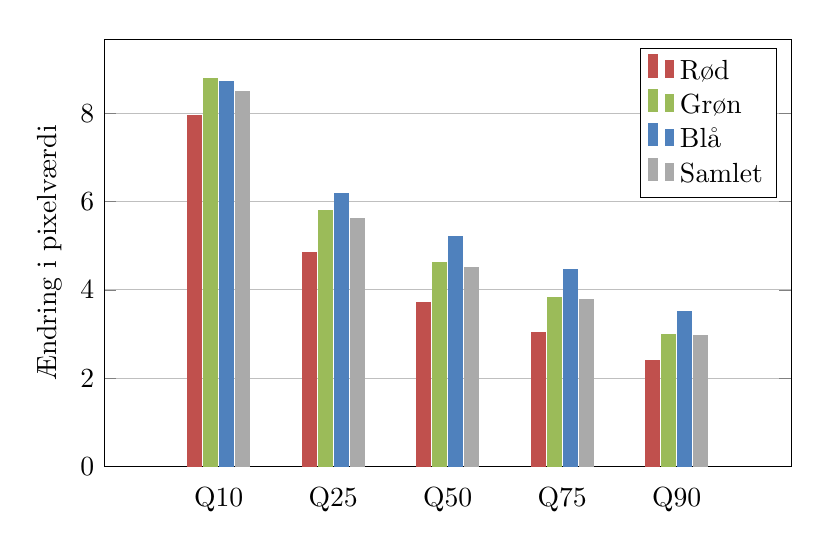
\begin{tikzpicture}
    \begin{axis}[
        width  = 0.85*\textwidth,
        height = 7cm,
        major x tick style = transparent,
        ybar=2*\pgflinewidth,
        bar width=5pt,
        ymajorgrids = true,
        ylabel = {Ændring i pixelværdi},
        symbolic x coords={Q10,Q25,Q50,Q75,Q90},
        xtick = data,
        scaled y ticks = false,
        enlarge x limits=0.25,
        ymin=0,
        legend cell align=left,
        legend style={
                %at={(1.25,0.0)},
                anchor=north east,
%                legend columns= -1,
%                /tikz/every even column/.append style= {column sep=1.0cm}
        }
    ]
        \addplot[style={rred,fill=rred,mark=none}]
            coordinates {(Q10, 7.95) (Q25,4.85) (Q50,3.71) (Q75,3.03) (Q90,2.39)};

        \addplot[style={ggreen,fill=ggreen,mark=none}]
             coordinates {(Q10, 8.79) (Q25,5.79) (Q50,4.62) (Q75,3.82) (Q90,2.99)};

        \addplot[style={bblue,fill=bblue,mark=none}]
             coordinates {(Q10, 8.73) (Q25,6.19) (Q50,5.21) (Q75,4.47) (Q90,3.51)};

        \addplot[style={ggray,fill=ggray,mark=none}]
             coordinates {(Q10, 8.49) (Q25,5.61) (Q50,4.51) (Q75,3.77) (Q90,2.96)};

        \legend{Rød, Grøn, Blå , Samlet}
    \end{axis}
\end{tikzpicture}
\caption{Gennemsnitlig ændring i pixelværdi med DCT \label{fig:pixelchange_DCT_diagram}}
\end{figure}
\begin{figure}[htbp]
\centering
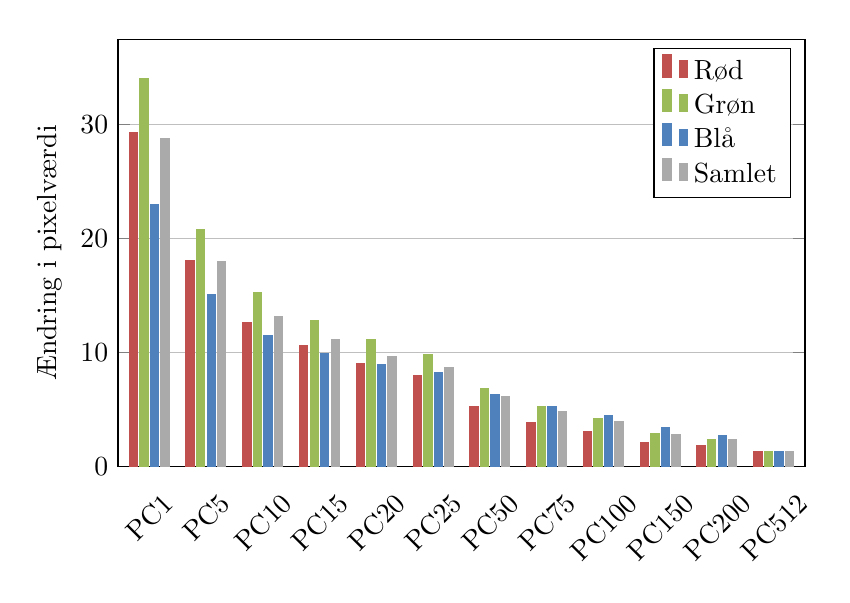
\begin{tikzpicture}
    \begin{axis}[
        width  = 0.85*\textwidth,
        height = 7cm,
        major x tick style = transparent,
        ybar=2*\pgflinewidth,
        bar width=3pt,
        ymajorgrids = true,
        ylabel = {Ændring i pixelværdi},
        symbolic x coords={PC1,PC5,PC10,PC15,PC20, PC25, PC50, PC75,PC100,PC150,PC200,PC512},
        xtick = data,
        x tick label style = {rotate = 45},
        scaled y ticks = false,
        enlarge x limits=0.05,
        ymin=0,
        legend cell align=left,
        legend style={
                %at={(0.0,-1.3)},
                anchor=north east,
%                legend columns= -1,
%                /tikz/every even column/.append style= {column sep=1.0cm}
        }
    ]
        \addplot[style={rred,fill=rred,mark=none}]
            coordinates {(PC1, 29.27) (PC5,18.05) (PC10,12.65) (PC15,10.64) (PC20,9.02) (PC25,7.95) (PC50, 5.25) (PC75,3.89) (PC100,3.10) (PC150,2.10) (PC200,1.85) (PC512,1.26)};

        \addplot[style={ggreen,fill=ggreen,mark=none}]
             coordinates {(PC1, 34.02) (PC5,20.75) (PC10,15.25)(PC15,12.79) (PC20,11.10) (PC25,9.84) (PC50,6.85) (PC75,5.28) (PC100,4.24) (PC150,2.90) (PC200,2.35) (PC512,1.27)};

        \addplot[style={bblue,fill=bblue,mark=none}]
             coordinates {(PC1, 22.98) (PC5,15.03) (PC10,11.44)(PC15,9.92) (PC20,8.89) (PC25,8.19) (PC50,6.26) (PC75,5.22) (PC100,4.48) (PC150,3.37) (PC200,2.75) (PC512,1.28)};

        \addplot[style={ggray,fill=ggray,mark=none}]
             coordinates {(PC1, 28.75) (PC5,17.95) (PC10,13.12)(PC15,11.12) (PC20,9.67) (PC25,8.66) (PC50,6.12) (PC75,4.79) (PC100,3.93) (PC150,2.79) (PC200,2.32) (PC512,1.27)};

        \legend{Rød, Grøn, Blå , Samlet}
    \end{axis}
\end{tikzpicture}
\caption{Gennemsnitlig ændring i pixelværdi med PCA \label{fig:pixelchange_PCA_diagram}}
\end{figure}

Det kan også være interessant at se på, hvor stor den største ændring i pixelværdi i de respektive komprimeringer, er. Dette giver bl.a. et udtryk for størrelsen af den ændring, som den pixel med største ændring oplever. Enkelte ændringer, der er meget store, kan lige så vel, som en stor gennemsnitlig ændring, blive tydelig for brugeren og fremstå som fejlfarvede pixels. Det må dog forventes, at disse afvigelser typisk vil være i forbindelse med bratte overgange i billedet.
Tabel \ref{tb:afvigelse_DCT} og \ref{tb:afvigelse_PCAl} præsenterer den største ændring i de forskellige farverum i alle komprimeringerne. Bemærk, at disse ændringer udtrykker den \emph{største} ændring, og dermed meget vel kun optræder meget få gange.

\begin{table}
\begin{minipage}[b]{0.45\textwidth}
\centering
\begin{tabular}{|l|l|l|l|}
\hline
	& \textbf{Rød}	& \textbf{Grøn}	& \textbf{Blå}	\\ \hline
\textbf{Q10}	& 110	& 124	& 110	\\ \hline
\textbf{Q25}	& 69		& 74		& 104	\\ \hline
\textbf{Q50}	& 48		& 62		& 87		\\ \hline
\textbf{Q75}	& 33		& 55		& 70		\\ \hline
\textbf{Q90}	& 22		& 39		& 43		\\ \hline
\end{tabular}
\caption{Største afvigelse for hver farve i DCT}
\label{tb:afvigelse_DCT}
\end{minipage}
\hspace{0.5cm}
\begin{minipage}[b]{0.45\textwidth}
\centering
\begin{tabular}{|l|c|c|c|}
\hline 
      & \textbf{Rød} & \textbf{Grøn} & \textbf{blå} 		  \\ \hline
\textbf{PC1}   & 136 & 185 & 135            \\ \hline
\textbf{PC5}   & 128 & 170 & 125            \\ \hline
\textbf{PC10}  & 121 & 171 & 123            \\ \hline
\textbf{PC15}  & 114 & 147 & 123            \\ \hline
\textbf{PC20}  & 105 & 136 & 117            \\ \hline
\textbf{PC25}  & 87  & 130 & 105            \\ \hline
\textbf{PC50}  & 59  & 96  & 88             \\ \hline
\textbf{PC75}  & 45  & 62  & 81             \\ \hline
\textbf{PC100} & 36  & 44  & 63             \\ \hline
\textbf{PC150} & 18  & 31  & 40             \\ \hline
\textbf{PC200} & 12  & 26  & 35             \\ \hline
\textbf{PC512} & 4   & 5   & 6              \\ \hline
\end{tabular}
\caption{Største afvigelse for hver farve i PCA}
\label{tb:afvigelse_PCAl}
\end{minipage}
\end{table}

Begrebet SNR blev introduceret i afsnit \vref{sec:stoj}, og er et udtryk for mængden af støj (afvigelser) i det dekomprimerede billede i forhold til det oprindelige billede. SNR udregnes som værende $SNR = \frac{\sigma^2_{\text{signal}}}{\sigma^{2}_{\text{støj}}}$, hvor prikproduktet beregnes som:
\begin{align}
\sigma^2_{\text{signal}} = \frac{1}{mn-1}  \tilde{\vec{x}}_{\text{signal}} \cdot \tilde{\vec{x}}_{\text{signal}}, \phantom{m} \text{hvor} \phantom{m} \tilde{\vec{x}}_{\text{signal}} = \vec{x}_{\text{signal}} - \mu_{x}
\end{align}
\begin{align}
\sigma^2_{\text{støj}} = \frac{1}{mn - 1} (\hat{\vec{x}} - \mu_{\hat{\vec{x}}}) \cdot (\hat{\vec{x}} - \mu_{\hat{\vec{x}}}), \phantom{m} \text{hvor} \phantom{m} \hat{\vec{x}} = \vec{x}_{\text{støj}} - \vec{x}_{\text{signal}}
\end{align}
SNR kan bruges som parameter til at vurdere kvaliteten af billedet. En høj SNR indikerer, at der er lidt støj, og billedet ligner dermed det oprindelige. Er SNR derimod lav, indikerer det en stor mængde støj, og dermed også at billedet er påvirket meget af støj, hvorved billedkvaliteten er dårlig. SNR udregnes for alle komprimeringerne i forhold til det oprindelige billede og er angivet i tabel \ref{tb:SNR_DCT} og \ref{tb:SNR_PCA}.

\begin{table}[htpb]
\begin{minipage}[b]{0.45\textwidth}
\centering
\begin{tabular}{|l|c|}
\hline
      & \textbf{SNR} \\ \hline
\textbf{Q10}   & 29,77                    \\ \hline
\textbf{Q25}   & 66,51                    \\ \hline
\textbf{Q50}   & 106,58                   \\ \hline
\textbf{Q75}   & 161,64                   \\ \hline
\textbf{Q90}   & 292,41                   \\ \hline
\end{tabular}
\caption{SNR for DCT-komprimeringer}
\label{tb:SNR_DCT}
\end{minipage}
\hspace{0.5cm}
\begin{minipage}[b]{0.45\linewidth}
\centering
\begin{tabular}{|l|c|}
\hline
& \textbf{SNR} \\ \hline
\textbf{PC1}	 & 2,46 \\ \hline
\textbf{PC5}	 & 5,80 \\ \hline
\textbf{PC10} & 10,13 \\ \hline
\textbf{PC15} & 14,26 \\ \hline
\textbf{PC20} & 18,91 \\ \hline
\textbf{PC25} & 23,68 \\ \hline
\textbf{PC50} & 53,04 \\ \hline
\textbf{PC75} & 95,39 \\ \hline
\textbf{PC100}& 155,38 \\ \hline
\textbf{PC150}& 346,31 \\ \hline
\textbf{PC200}& 639,82 \\ \hline
\textbf{PC512}& 7440,81 \\ \hline
\end{tabular}
\caption{SNR for PCA-komprimeringer}
\label{tb:SNR_PCA}
\end{minipage}
\end{table}


%Til sidst vises en graf med principal komponenternes udgørelse i procent i forhold til antal brugte principal components, se figur \ref{fig:PCAdiagram}. Dette er naturligvis en specifik graf for Lena-billedet.
%


%\begin{tikzpicture}
%    \begin{axis}[
%        width  = 0.85*\textwidth,
%        height = 8cm,
%        major x tick style = transparent,
%        ymajorgrids = true,
%        xmajorgrids=true,
%    		grid style=dashed,
%        ylabel = {Procent (\%)},
%		xlabel = {Principal Komponenter},
%        ymin=0,
%%		tick style={line width=5pt}
%        legend cell align=left,
%        legend style={
%                at={(0.12,-0.15)},
%                anchor=north west,
%                legend columns= -1,
%                /tikz/every even column/.append style= {column sep=1.0cm}}
%    ]
%        \addplot [ultra thick, blue] table [col sep=comma, mark = none] {PCA/data.csv};
%        \addplot [ultra thick, blue] table [col sep=comma, mark = none] {PCA/data.csv};
%
%%        \legend{Rød, Grøn, Blå , Samlet}
%    \end{axis}
%\label{fig:PCAdiagram}
%\end{tikzpicture}


%\begin{table}
%\centering
%\begin{tabular}{lrrrrr}
%\hline
%		&	Q10		&	Q25		&	Q50		&	Q75		&	%Q90		\\ \hline
%Rød		&	7,95	&	4,85	&	3,71	&	3,03	&	2,39	\\
%Grøn	&	8,79	&	5,80	&	4,62	&	3,82	&	2,99	\\
%Blå		&	8,73	&	6,19	&	5,21	&	4,47	&	3,51	\\ \hline
%Total	&	8,49	&	5,61	&	4,51	&	3,77	&	2,96	\\ \hline
%\end{tabular}
%\end{table}
%\fixme{denne tabel beskriver det samme som vores bar.plot vil vi gerne vise begge dele?}

Figur \ref{fig:PCAdiagram-EigenValues} viser, hvor mange procent hver egenværdi udgør for hele billedet i forhold til hver enkelt principal komponent. Dette betyder også, at man får en god idé om billedets indhold ved få principale komponenter. Diagrammet fortæller os til gengæld intet om den reelle billedkvalitet.

\begin{figure}[htbp]
\centering
\begin{tikzpicture}
    \begin{axis}[
        width  = 0.85*\textwidth,
        height = 8cm,
        ybar=2*\pgflinewidth,
        bar width=4pt,
        major x tick style = transparent,
        ymajorgrids = true,
%        xmajorgrids=true,
		y tick label style={/pgf/number format/.cd,
        scaled y ticks = false,
        set thousands separator={},
        %fixed
    		},
        ylabel = {Egenværdiernes andel af billedet [\%]},
		xlabel = {Principale komponenter},
        ymin=0,
%		tick style={line width=5pt}
        legend cell align=left,
        legend style={
                at={(0.12,-0.15)},
                anchor=north west,
                legend columns= -1,
                /tikz/every even column/.append style= {column sep=1.0cm}}
    ]
        \addplot [color=Peach, fill=Peach] table [col sep=comma, mark = none] {PCA/dataEigenProcent.csv};
    \end{axis}
%\label{fig:PCAdiagram-EigenValues}
\end{tikzpicture}
\caption{Procentudgørelse af billedet for hver egenværdi i forhold til hver principale komponent} \label{fig:PCAdiagram-EigenValues}
\end{figure}